\documentclass[10pt,a4paper]{article}
\usepackage[a4paper,margin=14mm,top=12mm,bottom=14mm]{geometry}
\usepackage{fontspec}
\setmainfont{Liberation Sans}
\usepackage{polyglossia}
\setdefaultlanguage{french}
\usepackage{amsmath}
\usepackage{xcolor}
\usepackage{graphicx}
\usepackage[most]{tcolorbox}
\usepackage{tabularx,booktabs,array,multirow}
\usepackage{enumitem}
\usepackage{fancyhdr}
\usepackage{lastpage}
\usepackage[hidelinks]{hyperref}
\definecolor{uimm}{HTML}{005677}
\definecolor{cyan}{HTML}{13A2DD}
\definecolor{fond}{HTML}{E6F2FA}
\definecolor{ok}{HTML}{2E7D32}
\definecolor{ko}{HTML}{B3261E}
\definecolor{violet}{HTML}{7B1FA2}
\setlength{\parindent}{0pt}
\setlength{\parskip}{3pt}
\setlist{nosep}
\setlist[itemize]{leftmargin=13pt,label=\textcolor{cyan}{\textbullet}}
\newcommand{\titre}[1]{\vspace{5pt}{\color{uimm}\large\bfseries #1}\par\vspace{-3pt}{\color{cyan}\rule{\linewidth}{1.2pt}}\par\vspace{0pt}}
\tcbset{boite/.style={colback=fond,colframe=uimm,boxrule=0.6pt,arc=2pt,left=6pt,right=6pt,top=4pt,bottom=4pt},
        defi/.style={colback=violet!6,colframe=violet,boxrule=0.8pt,arc=2pt,left=6pt,right=6pt,top=4pt,bottom=4pt,
                     title={\bfseries Défi},coltitle=white,colbacktitle=violet,fonttitle=\small}}
\newcommand{\bandeau}[3]{%
\begin{tcolorbox}[colback=uimm,colframe=uimm,arc=2pt,left=4pt,right=8pt,top=4pt,bottom=4pt]
\begin{minipage}[c]{18mm}\setlength{\fboxsep}{1.2pt}\fcolorbox{white}{white}{
\includegraphics[height=16.5mm]{logo_uimm.jpg}}\end{minipage}\hspace{4mm}%
\begin{minipage}[c]{\dimexpr\linewidth-22mm\relax}\color{white}
{\small #1}\\[1pt]{\LARGE\bfseries #2}\\[2pt]{\large #3}\hfill{\small CQPM Technicien qualité}
\end{minipage}
\end{tcolorbox}}
\newcommand{\reponse}[1][1]{\par\vspace{2pt}{\color{gray!60}\foreach \i in {1,...,#1}{\rule{\linewidth}{0.3pt}\par\vspace{9pt}}}}
\usepackage{pgffor}
\pagestyle{fancy}\fancyhf{}
\renewcommand{\headrulewidth}{0pt}
\newcommand{\pied}[1]{\fancyfoot[L]{\footnotesize\color{uimm}#1}\fancyfoot[R]{\footnotesize\color{uimm}Page \thepage{} sur \pageref{LastPage}}}

\usepackage{tikz}
\usepackage{longtable}
\renewcommand{\bandeau}[3]{%
\begin{tcolorbox}[colback=uimm,colframe=uimm,arc=2pt,left=4pt,right=8pt,top=4pt,bottom=4pt]
\begin{minipage}[c]{18mm}\setlength{\fboxsep}{1.2pt}\fcolorbox{white}{white}{
\includegraphics[height=16.5mm]{logo_uimm.jpg}}\end{minipage}\hspace{4mm}%
\begin{minipage}[c]{\dimexpr\linewidth-22mm\relax}\color{white}
{\small #1}\\[1pt]{\LARGE\bfseries #2}\\[2pt]{\large #3}
\end{minipage}
\end{tcolorbox}}
% en-tête d'une fiche : code, titre, question, bloc, durée, organisation, niveau
\newcommand{\entete}[7]{%
\begin{tcolorbox}[colback=uimm,colframe=uimm,arc=2pt,left=4pt,right=6pt,top=4pt,bottom=4pt]
\begin{minipage}[c]{18mm}\setlength{\fboxsep}{1.2pt}\fcolorbox{white}{white}{
\includegraphics[height=16.5mm]{logo_uimm.jpg}}\end{minipage}\hspace{3mm}%
\begin{minipage}[c]{\dimexpr\linewidth-58mm\relax}\color{white}\raggedright
{\small Base SPC · #4}\\[1pt]{\Large\bfseries #1 · #2}\\[2pt]{\itshape #3}
\end{minipage}\hfill
\begin{minipage}[c]{33mm}\color{white}\small\raggedleft
Durée : \textbf{#5}\\ \textbf{#6}\\ Niveau #7 sur 3
\end{minipage}
\end{tcolorbox}}
\newcommand{\tagE}{{\setlength{\fboxsep}{1.5pt}\colorbox{cyan}{\color{white}\scriptsize\bfseries Ellistat}}}
\newcommand{\tagW}{{\setlength{\fboxsep}{1.5pt}\colorbox{uimm}{\color{white}\scriptsize\bfseries Page web}}}
\tcbset{pred/.style={colback=orange!6,colframe=orange!80!black,boxrule=0.6pt,arc=2pt,left=6pt,right=6pt,top=3pt,bottom=1pt,
                    title={\bfseries Je prédis, avant de commencer},coltitle=white,colbacktitle=orange!80!black,fonttitle=\small},
        retenir/.style={colback=fond,colframe=uimm,boxrule=0.6pt,arc=2pt,left=6pt,right=6pt,top=3pt,bottom=3pt,
                    title={\bfseries À retenir},coltitle=white,colbacktitle=uimm,fonttitle=\small},
        plus/.style={colback=violet!6,colframe=violet,boxrule=0.6pt,arc=2pt,left=6pt,right=6pt,top=3pt,bottom=3pt,
                    title={\bfseries Pour aller plus loin},coltitle=white,colbacktitle=violet,fonttitle=\small},
        act/.style={colback=uimm!10,colframe=uimm,boxrule=0.5pt,arc=2pt,left=5pt,right=5pt,top=2pt,bottom=2pt,before skip=7pt,after skip=3pt},
        verif/.style={colback=orange!6,colframe=orange!80!black,boxrule=0.6pt,arc=2pt,left=6pt,right=6pt,top=3pt,bottom=3pt,
                    title={\bfseries À vérifier sur poste avant la première séance},coltitle=white,colbacktitle=orange!80!black,fonttitle=\small}}
\newcommand{\fichier}[1]{\texttt{\small #1}}
\newcommand{\menu}[1]{\textsf{\textbf{#1}}}
\newcommand{\champ}[1]{\rule{#1}{0.3pt}}

\pied{Base SPC · fiche G3 · Le nominal n'est pas le milieu}
\begin{document}
\thispagestyle{fancy}
\entete{G3}{Le nominal n'est pas le milieu}{Ma cote est-elle centrée dans sa tolérance ?}{Mallettes GUNT : plaques et arbres}{45 min}{en groupe}{2}
\begin{tcolorbox}[boite]\textbf{Le but.} Lire une tolérance dissymétrique sur l'arbre PT105 (cotes b = 30,3 +0,4 et d = 55,2 −0,4), mesurer 20 arbres, et constater que le nominal n'est pas le milieu de la tolérance : le Ppk le dit.\par\textbf{Il vous faut.} 20 arbres PT105 numérotés · Un pied à coulisse par binôme · Le plan de l'arbre (dernière page de la fiche) · Ellistat\end{tcolorbox}
\begin{tcolorbox}[pred]Le tour vise le nominal : 30,3 pour $b$ et 55,2 pour $d$. Sur 20 arbres, combien seront hors tolérance pour chacune des deux cotes ?\reponse\end{tcolorbox}
\titre{À faire}
\begin{enumerate}[label=\textcolor{cyan}{\textbf{\arabic*.}},leftmargin=15pt,itemsep=1.5pt]
\item Lire sur le plan (dernière page) la tolérance de $b$ et de $d$ (un seul écart est écrit : l'autre vaut zéro). Compléter le premier tableau : limites, milieu, $T$.
\item Répartir les 20 arbres entre les binômes. Mesurer $b$ et $d$ de chaque arbre au pied à coulisse et noter dans le second tableau. Réunir les 20 valeurs de chaque cote dans la même grille.
\item \tagE\ Coller les valeurs dans deux colonnes de la grille. Panneau de colonne, onglet \menu{Informations} : \menu{Nom}, \menu{Nb décimales} 2, \menu{Tolerance min} et \menu{Tolerance max} avec les \textbf{vraies} limites (comme en E3).
\item \tagE\ \menu{Stats Desc.}, \menu{Détail}, cocher la colonne de $b$ : histogramme, tableaux \menu{PARAMÈTRES}, \menu{CAPABILITÉ} (Pp, Ppk) et \menu{\% HORS TOLÉRANCE}. Même chose pour $d$.
\item \tagE\ Pour $b$, remplacer Tolerance min par 29,9 et Tolerance max par 30,7 (lecture « 30,3 $\pm$ 0,4 » : un piège classique). Relire Pp et Ppk, puis remettre les vraies limites.
\item À la main : où faut-il viser la moyenne pour que Ppk égale Pp ? De combien faut-il la décaler ?
\end{enumerate}
\vspace{3pt}{\renewcommand{\arraystretch}{1.5}\small\begin{tabularx}{\linewidth}{|l|*{5}{>{\centering\arraybackslash}X|}}\hline
\textbf{Cote} & \textbf{Nominal} & \textbf{Limite basse} & \textbf{Limite haute} & \textbf{Milieu} & \textbf{$T$}\\\hline
b & & & & & \\\hline
d & & & & & \\\hline
\end{tabularx}}\par\vspace{5pt}
\begin{minipage}[t]{0.485\linewidth}\textbf{Cote b (mm)}\par\vspace{2pt}
{\renewcommand{\arraystretch}{1.4}\begin{tabularx}{\linewidth}{|*{3}{>{\centering\arraybackslash}p{5mm}|>{\centering\arraybackslash}X|}}\hline
\scriptsize 1 &  & \scriptsize 2 &  & \scriptsize 3 & \\\hline
\scriptsize 4 &  & \scriptsize 5 &  & \scriptsize 6 & \\\hline
\scriptsize 7 &  & \scriptsize 8 &  & \scriptsize 9 & \\\hline
\scriptsize 10 &  & \scriptsize 11 &  & \scriptsize 12 & \\\hline
\scriptsize 13 &  & \scriptsize 14 &  & \scriptsize 15 & \\\hline
\scriptsize 16 &  & \scriptsize 17 &  & \scriptsize 18 & \\\hline
\scriptsize 19 &  & \scriptsize 20 &  &  & \\\hline
\end{tabularx}}\end{minipage}\hfill\begin{minipage}[t]{0.485\linewidth}\textbf{Cote d (mm)}\par\vspace{2pt}
{\renewcommand{\arraystretch}{1.4}\begin{tabularx}{\linewidth}{|*{3}{>{\centering\arraybackslash}p{5mm}|>{\centering\arraybackslash}X|}}\hline
\scriptsize 1 &  & \scriptsize 2 &  & \scriptsize 3 & \\\hline
\scriptsize 4 &  & \scriptsize 5 &  & \scriptsize 6 & \\\hline
\scriptsize 7 &  & \scriptsize 8 &  & \scriptsize 9 & \\\hline
\scriptsize 10 &  & \scriptsize 11 &  & \scriptsize 12 & \\\hline
\scriptsize 13 &  & \scriptsize 14 &  & \scriptsize 15 & \\\hline
\scriptsize 16 &  & \scriptsize 17 &  & \scriptsize 18 & \\\hline
\scriptsize 19 &  & \scriptsize 20 &  &  & \\\hline
\end{tabularx}}\end{minipage}\par
\newpage
\titre{J'observe, je décide}
\begin{enumerate}[label=\textcolor{cyan}{\textbf{Q\arabic*.}},leftmargin=22pt]
\item Milieu de la tolérance de $b$ : \champ{14mm} ; moyenne mesurée : \champ{14mm}. Même chose pour $d$ : \champ{14mm} et \champ{14mm}. Le nominal est-il le milieu ?\reponse[1]
\item Pp et Ppk de $b$ avec les vraies limites : \champ{12mm} et \champ{12mm}. Avec la mauvaise lecture : \champ{12mm} et \champ{12mm}. Que conclure ?\reponse[2]
\item Pour $d$ : de quel côté sort-on de la tolérance ? Combien d'arbres, sur 20 ?\reponse[1]
\item Pp est-il suffisant ? Que faut-il régler en premier sur le tour : la dispersion ou le centrage ?\reponse[2]
\end{enumerate}
\begin{tcolorbox}[retenir]Le nominal n'est pas toujours le milieu de la tolérance. Avec une tolérance dissymétrique, viser le nominal décentre le procédé : Pp est bon, Ppk est mauvais.\end{tcolorbox}
\providecommand{\carre}{\fbox{\rule{0pt}{1.1ex}\rule{1.1ex}{0pt}}}
\begin{tcolorbox}[boite,left=5pt,right=5pt,top=3pt,bottom=3pt]\footnotesize
\textbf{\color{uimm}Lire le plan GUNT (dernière page).} Le cartouche du plan est écrit en allemand et en anglais. À la ligne « Allgemeintoleranzen / General tolerance », on lit \textbf{ISO 2768-mK}. Cela veut dire : toute cote \textbf{sans écart écrit} a la tolérance générale de la classe \textbf{m} (« medium »), donnée par le tableau ci-dessous. Une cote \textbf{avec un écart écrit} garde cet écart, et la tolérance générale ne s'applique pas. Limite haute = nominal + écart supérieur. Limite basse = nominal + écart inférieur. \O\ : diamètre. \carre{} : carré, on lit son côté. « A-A », « B-B » : coupes. Les symboles d'état de surface et d'arêtes, en bas à droite, ne servent pas dans cette fiche.
\par\vspace{6pt}\noindent\renewcommand{\arraystretch}{1.2}\setlength{\tabcolsep}{4pt}
\begin{tabular}{|l|c|c|c|c|c|}\hline
\textbf{Dimension nominale (mm)} & 0,5 à 3 & au-delà de 3 à 6 & au-delà de 6 à 30 & au-delà de 30 à 120 & au-delà de 120 à 400\\\hline
\textbf{Écart de la classe m (mm)} & $\pm 0{,}1$ & $\pm 0{,}1$ & $\pm 0{,}2$ & $\pm 0{,}3$ & $\pm 0{,}5$\\\hline
\end{tabular}
\par\vspace{1pt}{\scriptsize Source : ISO 2768-1:1989, tolérances générales des dimensions linéaires, reprises dans la fiche GUNT « PT105f Tolérances ».}
\par\vspace{4pt}\textbf{Les cotes de cette fiche}\par\vspace{2pt}
\begin{tabularx}{\linewidth}{|c|>{\raggedright\arraybackslash}X|>{\raggedright\arraybackslash}X|}\hline
\textbf{Cote} & \textbf{Ce que le plan écrit} & \textbf{Écart à utiliser}\\\hline
$b$ & 30,3 avec $+0{,}4$ (un seul écart écrit) & convention de cette fiche : l'autre écart vaut $0$ \\\hline
$d$ & 55,2 avec $-0{,}4$ (un seul écart écrit) & convention de cette fiche : l'autre écart vaut $0$ \\\hline
\end{tabularx}
\end{tcolorbox}
\vfill{\footnotesize\color{uimm}\textbf{Ressources de la base :} Données de secours : \href{https://sjaubert.github.io/000_OI/SPC/Pages/Donnees_a_copier.html\#decentre}{\nolinkurl{https://sjaubert.github.io/000_OI/SPC/Pages/Donnees_a_copier.html}}}
\newpage
\titre{Plan de l'arbre PT105}
{\small Pour lire ce plan et ses tolérances, voir l'encadré « Lire le plan GUNT » de la page précédente.\par}\vspace{2pt}
\begin{center}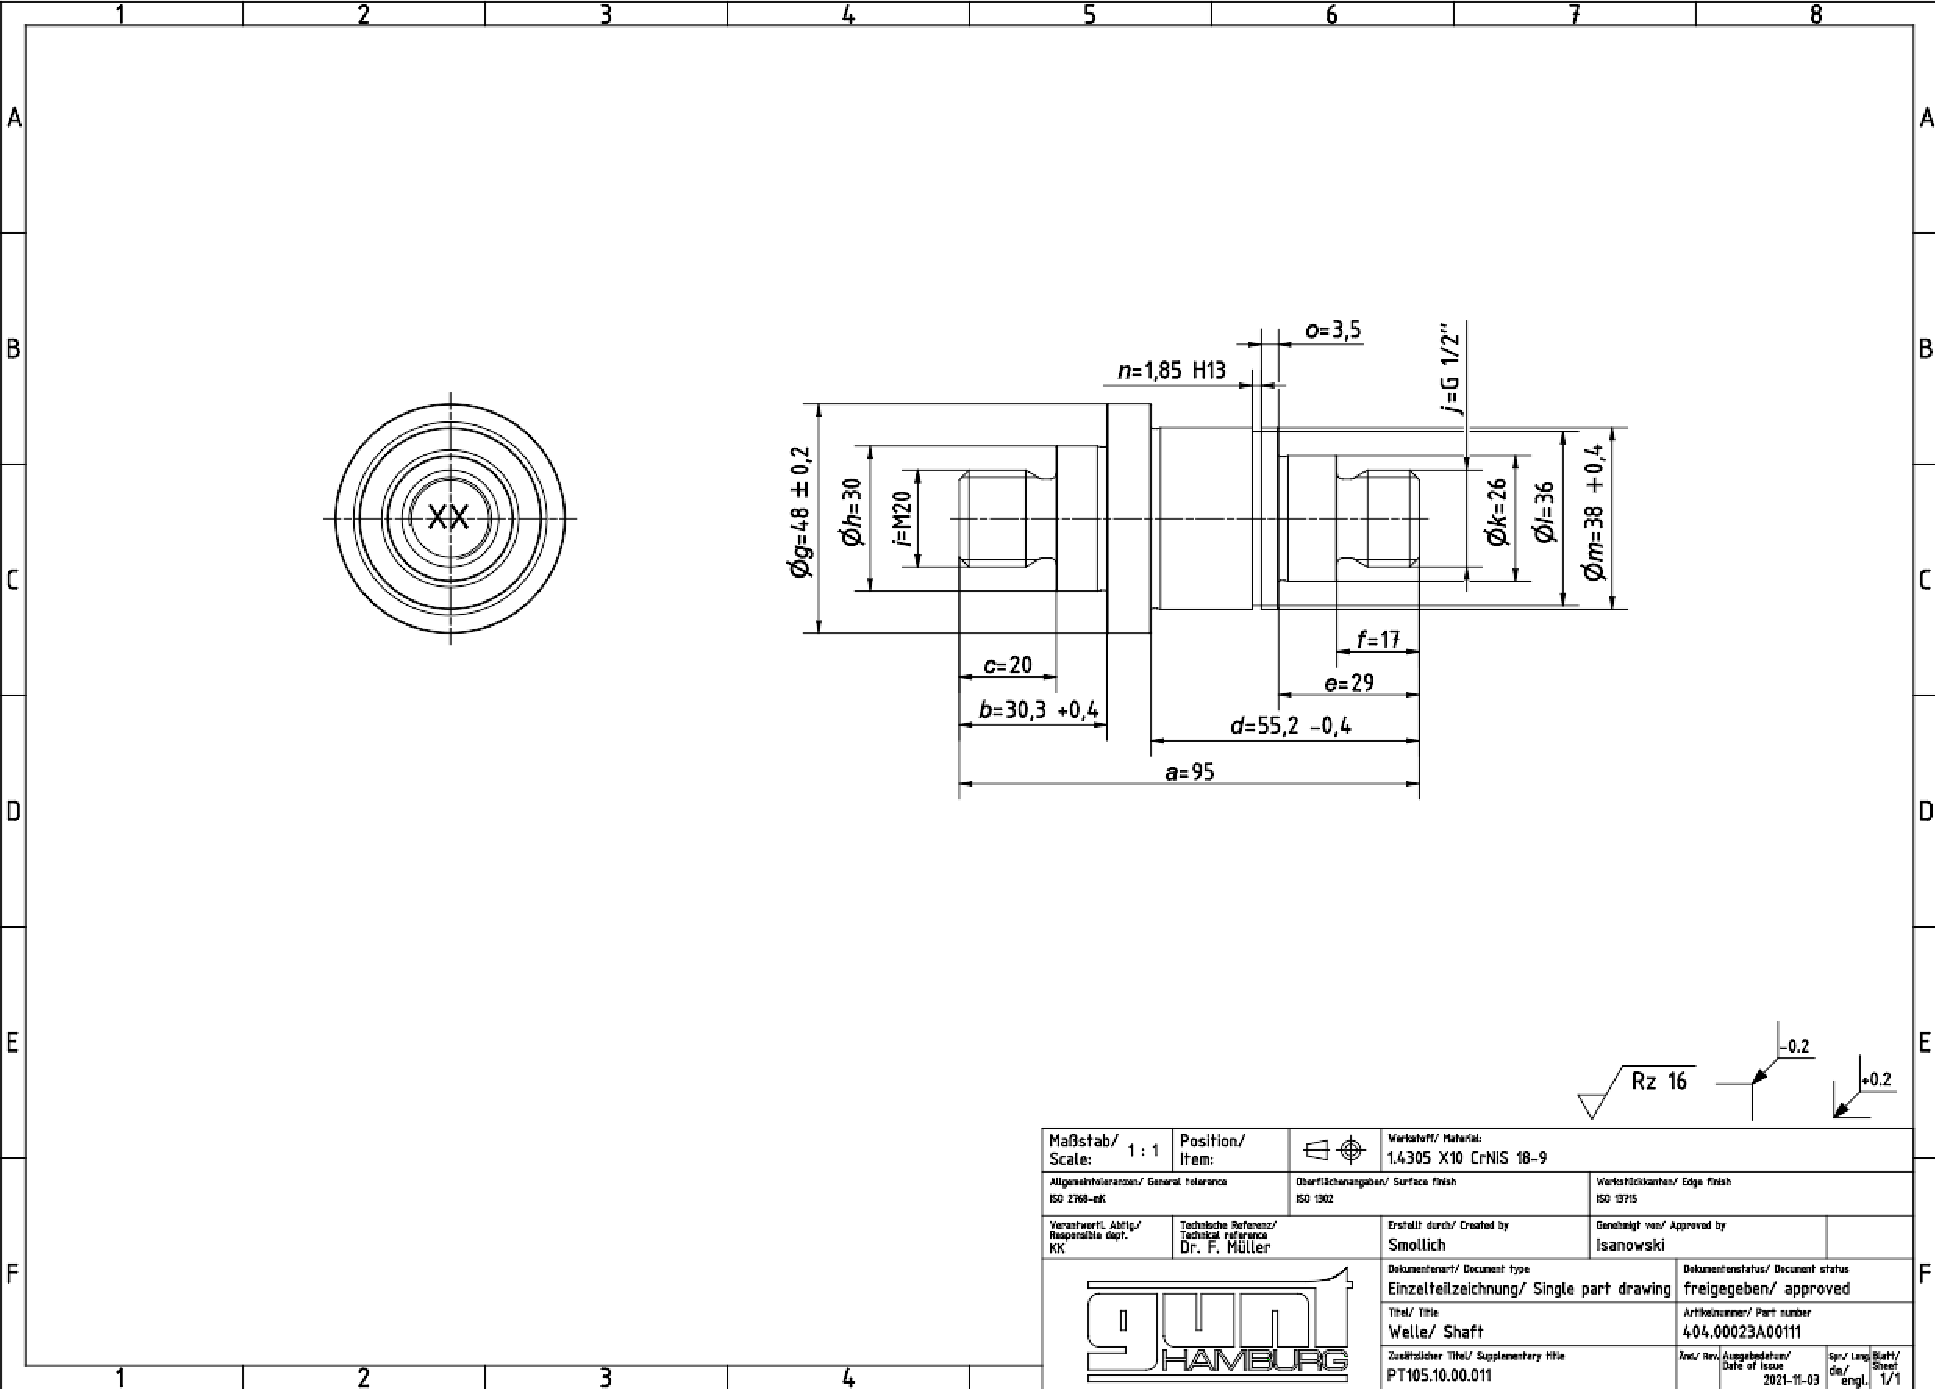
\includegraphics[width=0.90\textheight,height=0.97\linewidth,keepaspectratio,angle=90]{plan_arbre_PT105.pdf}\end{center}
\vfill{\footnotesize\color{uimm}Plan : GUNT Hamburg, Welle (arbre), dessin PT105.10.00.011.}
\end{document}